\clearpage

\section{Quantum Phenomena and Entanglement}
\label{sec:quantum-phenomena-and-entanglement}

Building on the non-injectivity of the projection~$\Pi$
(Section~\ref{subsec:relational-projection}), this section shows how
entanglement, nonlocal correlations, measurement statistics, and the
formal apparatus of quantum mechanics emerge without introducing
additional ontological degrees of freedom.
The framework adopts \textbf{ontological monism}: there is a single
ontological substrate~$\chi$, while apparent multiplicity and spatial
separation are properties of the projected description.

\input{4-quantum_mechanics/08-quantum_phenomena_and_entanglement/001-non-injective-projection}
\subsection{Nonlocality and the Holistic Character of Projected Descriptions}
\label{subsec:nonlocality-and-holistic-nature}

Quantum nonlocality does not arise from superluminal interactions but
reflects the intrinsically non-factorizable character of certain admissible projected descriptions~\cite{Bell1964}.
Entangled systems correspond to single projected configurations that
cannot be decomposed into independent subsystems without loss of admissibility.

\subsection{Nonlocal Correlations Without Superluminality}
\label{subsec:nonlocal-correlations-without-superluminality}

Correlated outcomes arise because spacelike separated measurements
correspond to different local reprojections of a single non-factorizable
description.
The factorization assumptions underlying Bell-type inequalities are
violated, while dynamical locality and relativistic causality remain
intact (see
Appendix~\ref{subsec:non-factorization-entanglement}).
The correlations are \emph{ontological}---fixed by the non-injective
global relational structure---rather than \emph{dynamical}.

Attosecond-resolved measurements have demonstrated that quantum
correlations become experimentally accessible on timescales far shorter
than any interaction-based
mechanism~\cite{PhysRevLett.133.163201}.
Within Cosmochrony, the observed timescale corresponds to the resolution
time of the effective projection~$\Pi$, not to a physical propagation
time: it probes projective accessibility rather than dynamical formation
of correlations.

\subsection{Temporal Ordering and Relativistic Consistency}
\label{subsec:temporal-ordering-and-relativistic-consistency}

Temporal ordering arises only at the effective level.
Different observers may assign different orderings to spacelike separated
events; such differences reflect observer-dependence of spacetime slicing
and have no impact on the relational consistency of admissible descriptions.
Relativistic covariance is preserved by the invariance of the underlying
non-injective relational configuration across all admissible projected descriptions.

\subsection{Relation to Bell Inequalities}
\label{subsec:relation-to-bell-inequalities}

Bell's theorem~\cite{Bell1964} rules out any ontological completion of
quantum mechanics based on factorizable hidden-variable models.
Cosmochrony fully accepts Bell's theorem and identifies the ontological
assumption that fails: the factorization hypothesis $P(a,b|x,y,\lambda) = P(a|x,\lambda)\,P(b|y,\lambda)$.

Because the projection~$\Pi$ is generically non-injective, admissible
projected states are not associated with independent ontic pre-images for their subsystems.
The factorization hypothesis is not merely violated but \emph{ill-defined}
within the space of admissible projected descriptions.

Bell-type violations arise in an intermediate regime of projective
compression: the effective description is sufficiently coarse-grained to
permit subsystem separation, yet retains enough global relational structure to prevent factorization.
In the limit of extreme coarse-graining, projected descriptions become effectively classical.

\begin{figure}[t]
  \centering
  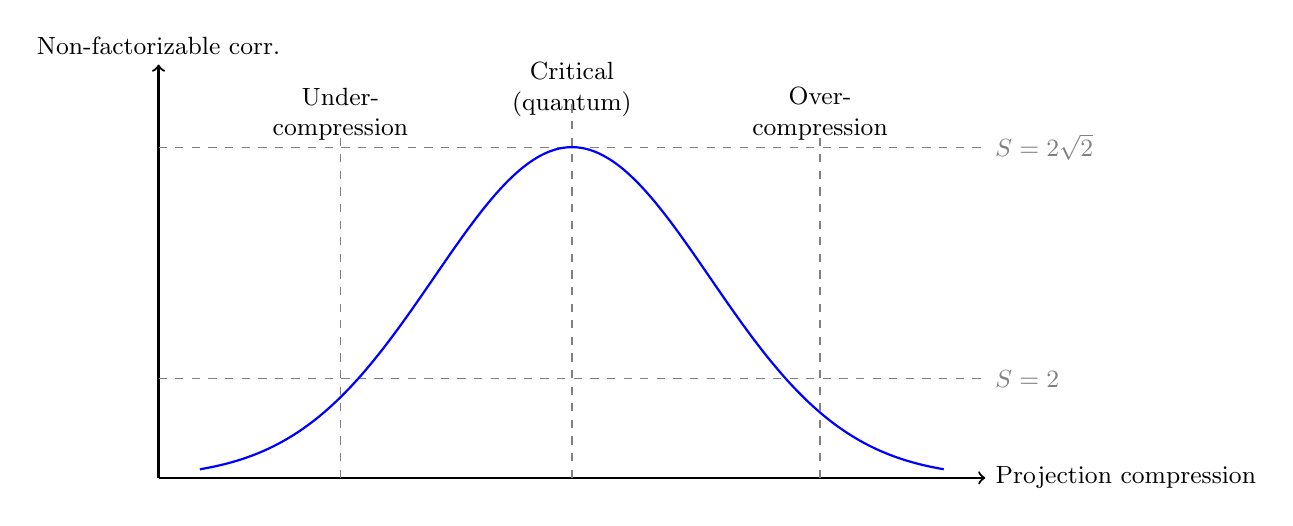
\begin{tikzpicture}[
    scale=1.05,
    axis/.style={->, thick},
    curve/.style={thick, smooth, blue},
    dashedline/.style={dashed, gray},
    label/.style={font=\small}
  ]
    \draw[axis] (0,0) -- (10,0)
      node[right,label] {Projection compression};
    \draw[axis] (0,0) -- (0,5)
      node[above,label] {Non-factorizable corr.};
    \draw[dashedline] (0,1.2) -- (10,1.2)
      node[right,label] {$S=2$};
    \draw[dashedline] (0,4) -- (10,4)
      node[right,label] {$S=2\sqrt{2}$};
    \draw[curve]
      plot[domain=0.5:9.5,samples=200]
      (\x,{4*exp(-0.18*(\x-5)^2)});
    \node[label, align=center] at (2.2,4.4)
      {Under-\\compression};
    \node[label, align=center] at (5,4.7)
      {Critical\\(quantum)};
    \node[label, align=center] at (8,4.4)
      {Over-\\compression};
    \draw[dashedline] (2.2,0) -- (2.2,4.2);
    \draw[dashedline] (5,0) -- (5,4.6);
    \draw[dashedline] (8,0) -- (8,4.2);
  \end{tikzpicture}
  \caption{Bell inequality violations as a function of the
    compression induced by~$\Pi$.
    Non-factorizable correlations emerge in an intermediate regime.}
  \label{fig:bell-compression-regime}
\end{figure}

No hidden variables and no superluminal influence are introduced.
Quantum nonlocality is ontological rather than dynamical: the failure of
Bell-type factorizability arises from the structure of admissible projected descriptions, not from nonlocal interaction.

\subsection{Measurement, Decoherence, and Apparent Collapse}
\label{subsec:measurement-and-decoherence}

Quantum measurement does not involve fundamental wavefunction collapse.
Measurement corresponds to the transition from a non-factorizable
admissible projected description to a set of effectively factorized local projections.
Decoherence suppresses interference between incompatible descriptive
branches by rendering their relative phase information inaccessible
within spacetime representations~\cite{Zurek2003}.
The underlying relational structure remains globally well defined.
The apparent collapse is the effective manifestation of a non-injective
relational structure becoming only partially projectable into spacetime.

\subsection{Limits of Entanglement and Environmental Effects}
\label{subsec:limits-of-entanglement}

Entanglement arises only within restricted regimes in which a
non-factorizable global description remains jointly projectable.
Environmental coupling progressively restricts the set of admissible
projected descriptions to locally stable, approximately factorizable regimes.
Entanglement is most robust for effectively isolated systems and becomes
increasingly fragile in macroscopic environments.
Classical behavior emerges when only factorized projected descriptions
remain admissible, without requiring any modification of the underlying relational structure.

\input{4-quantum_mechanics/08-quantum_phenomena_and_entanglement/008-structural-stability}
\subsection{Entanglement as a Critical Regime of Projective Compression}
\label{subsec:entanglement-critical-compression}

Quantum entanglement arises as a structural consequence of the non-injective
projection $\Pi:\chi \rightarrow \chi_{\mathrm{eff}}$.
The projection reduces a high-dimensional relational configuration to a
lower-dimensional effective description; the resulting fiber $\Pi^{-1}(\chi_{\mathrm{eff}})$ constitutes an
  information-theoretic channel whose bandwidth depends on unresolved modes of~$\chi$.

Non-factorizable correlations emerge only in an intermediate
\emph{critical} regime of projective compression: the effective
description is sufficiently coarse-grained to permit subsystem
identification, yet retains enough global relational structure to prevent full factorization.
Increased compression (environmental coupling, decoherence) suppresses
correlations, yielding classical behavior; decreased compression breaks subsystem separation.
The critical regime may be intermittent, with correlations appearing
during specific spectral reconfiguration events (Appendix~\ref{sec:appendix-simulation}).

\input{4-quantum_mechanics/08-quantum_phenomena_and_entanglement/010-implications-quantum-computation}
\input{4-quantum_mechanics/08-quantum_phenomena_and_entanglement/011-standard-model}
\input{4-quantum_mechanics/08-quantum_phenomena_and_entanglement/012-quantum-formalism}
% ----------------------------------------------------------------------------
% Section 8.9 --- Summary
% From former §8.12, condensed
% ----------------------------------------------------------------------------
\subsection{Summary}
\label{subsec:summary-quantum}

Gauge interactions emerge as admissible modes of the projection process.
The photon corresponds to scalar transmission modes; $W^\pm$ and $Z^0$
bosons arise as shear-like spectral modes whose masses reflect the
spectral rigidity of the projection fiber.
Strong interactions and confinement are reinterpreted through topological
stability of knotted solitonic configurations.
Mass emerges from spectral overlap between localized configurations and
the global relaxation flux.
Entanglement and nonlocal correlations reflect the persistence of
non-factorizable admissible projected descriptions.
Quantum mechanics appears as an effective statistical framework
describing the limits of local projectability imposed by a globally
non-injective relational structure.
Classical behavior emerges as the limiting case in which only locally
stable, factorizable projected descriptions remain admissible.

